\subsection{OLR, PM2.5, and Ring: Complete Temporal Maps}\label{sec:remaining_temporal}
\begin{figure*}[t]
\centering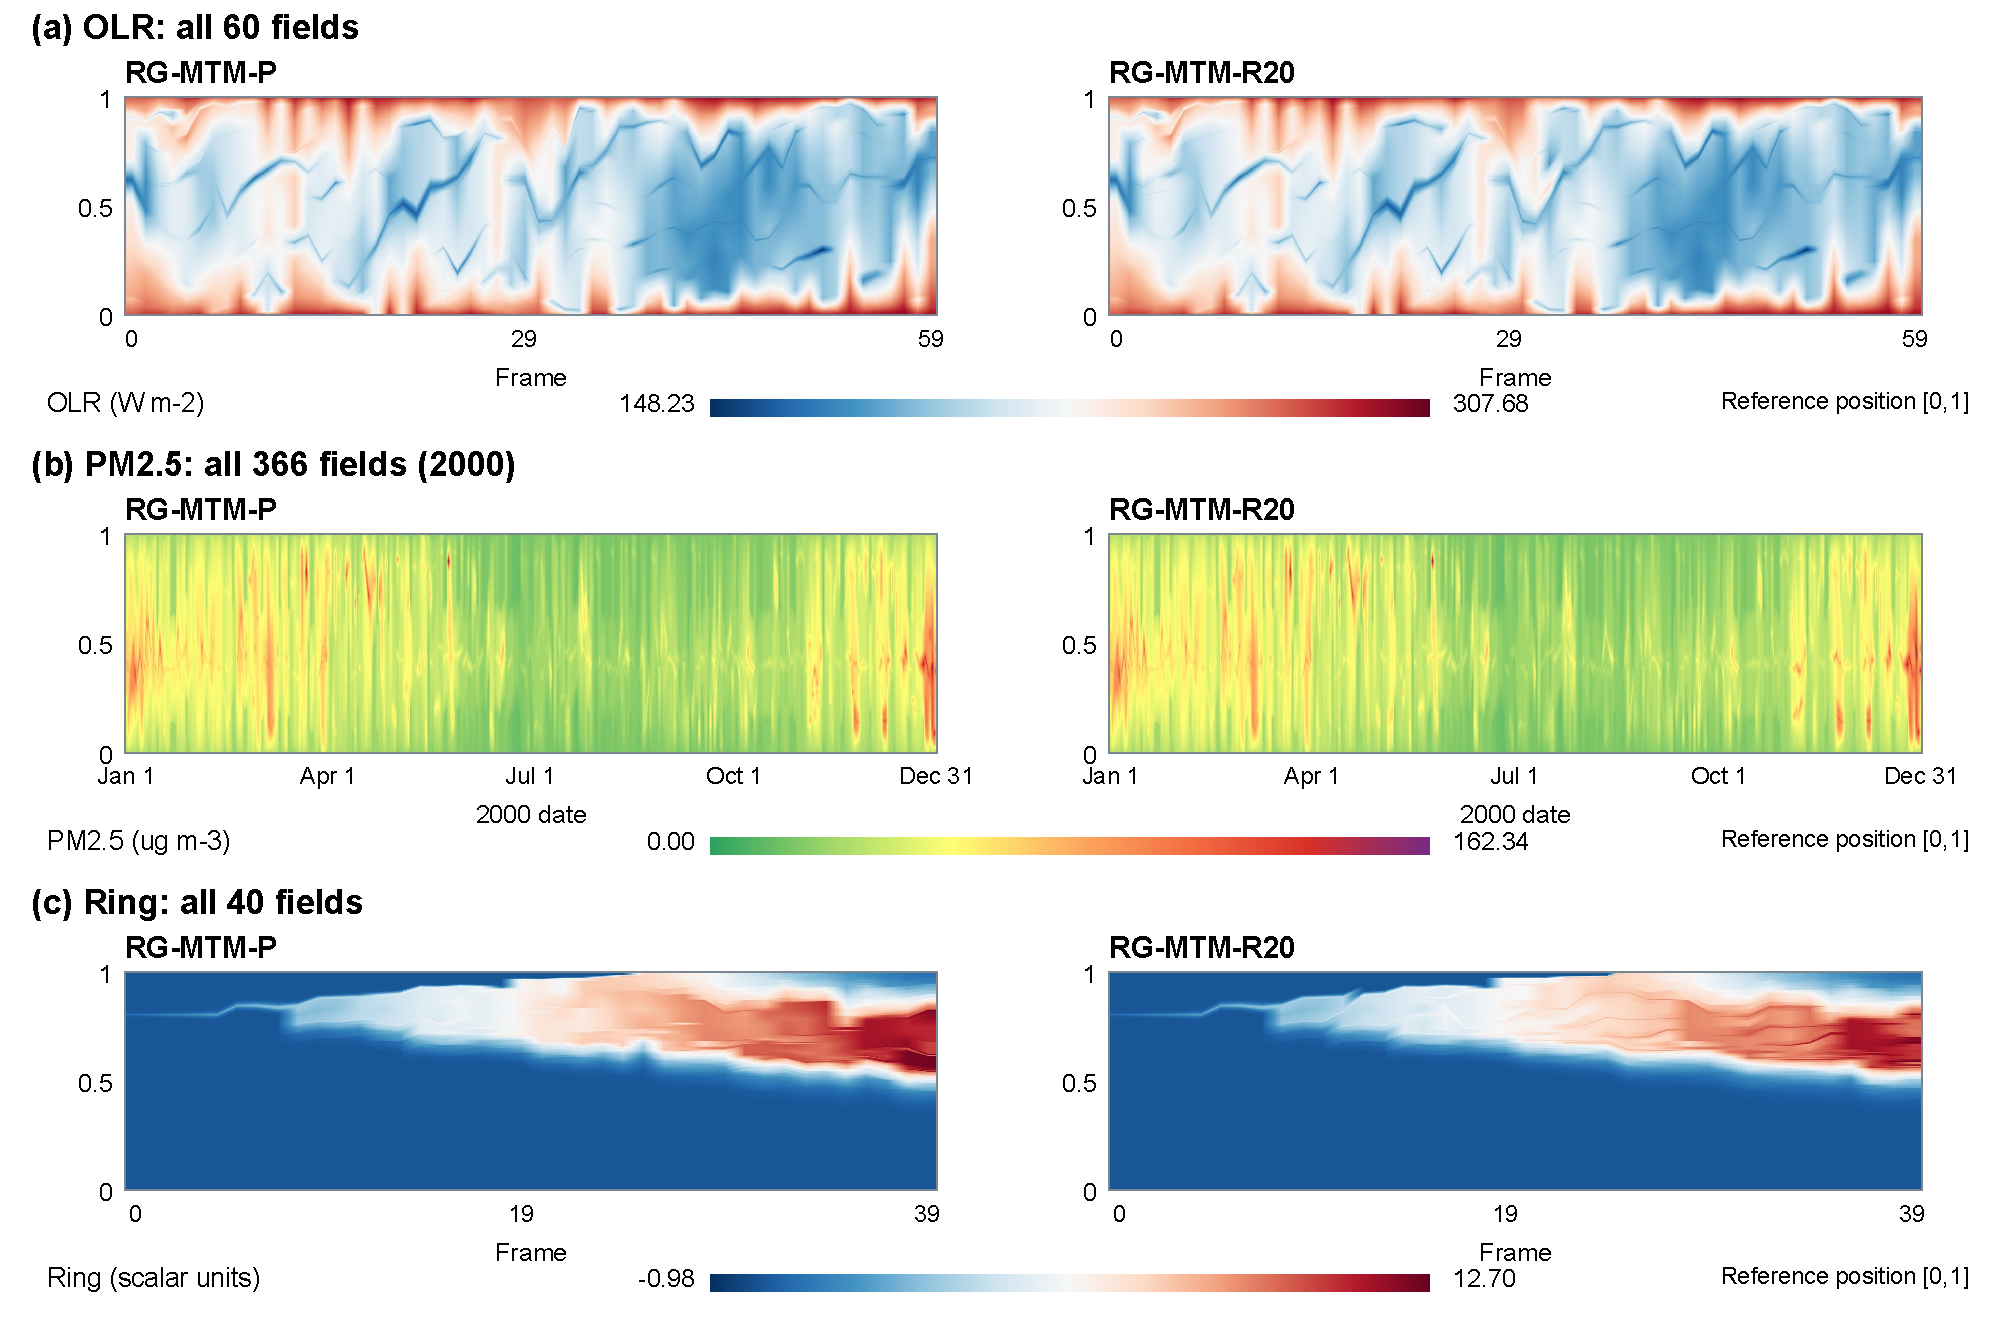
\includegraphics[width=\textwidth]{figures/Fig12.pdf}
\caption{Complete P/R20 temporal maps for three additional inputs: (a) OLR, all 60 daily fields; (b) PM2.5, all 366 fields in 2000; (c) Ring, all 40 synthetic fields. Horizontal axes show frames; vertical axes show the same normalized fixed reference within each P/R pair. Scalar ranges are shared within each row and independent between datasets. Maps use complete sequences without temporal cropping. Conservative display interpolation preserves each saved profile exactly; intermediate columns do not add observations. PM2.5 uses the user-authorized green--yellow--orange--red--purple pollution palette in concentration units, without AQI thresholds. Colours encode processed scalar values; any below-input-range connections are layout outputs. Complete arrays, not preview pixels, determine the reported errors. The complete four-method comparisons are in Supplement S10.}
\label{fig:remaining_temporal}
\end{figure*}

Figure~\ref{fig:remaining_temporal} completes the direct result coverage of all nine inputs. It shows all 60 OLR fields, all 366 PM2.5 fields in 2000, and all 40 Ring fields for P and R20. Each pair shares one fixed reference axis and scalar scale. Supplement S10 retains complete four-method comparisons with the baselines' native ordinates.

OLR NROE decreases from P's 0.89\% to zero, while motion errors remain 3/56. Annual PM2.5 NROE decreases from 0.9785\% to 0.0074\%; pooled displacement decreases from 1.87\% to 0.76\%, at 0.182\% mean and 4.669\% maximum NMLE. However, motion errors increase from 42/95 to 47/95. The complete year therefore supports reference alignment rather than a general improvement in spatial motion. January's selected seven-event example is retained only as a historical control. Ring reduces NROE from 2.66\% to 0.13\% and motion errors from 39/124 to 16/124, at 2.73\% mean NMLE.

Map appearance depends on temporal sampling, the number of retained extrema, and scalar filling. A frame with one or two extrema naturally contains broad bands; the full year adds observed temporal coverage without inventing additional features. For display in Figures~\ref{fig:fire_events}, \ref{fig:volume}, \ref{fig:cylinder}, \ref{fig:remaining_temporal}, and \ref{fig:pm25_case}, we interpolate neighbouring saved profiles with a monotone warp aligned to common extrema when order and displacement permit, otherwise using fixed-position linear interpolation. Every saved scalar profile remains exact at its frame before pixel rendering, and no scalar overshoot is introduced. For the Wildfires, Tangaroa, and Cylinder revisions, vertical area antialiasing integrates all stored rendering rows. The actual FRP cell polygons retain their discrete geometry. Intermediate columns are display samples, not additional observations, layouts, or temporal evidence. All numerical results use the original saved frames.
